\documentclass{beamer}
\usepackage[utf8]{inputenc}

\usetheme{Madrid}
\usecolortheme{default}
\usepackage{amsmath,amssymb,amsfonts,amsthm}
\usepackage{mathtools}
\usepackage{txfonts}
\usepackage{tkz-euclide}
\usepackage{listings}
\usepackage{adjustbox}
\usepackage{tfrupee}
\usepackage{array}
\usepackage{gensymb}
\usepackage{tabularx}
\usepackage{gvv}
\usepackage{lmodern}
\usepackage{circuitikz}
\usepackage{tikz}
\lstset{literate={·}{{$\cdot$}}1 {λ}{{$\lambda$}}1 {→}{{$\to$}}1}
\usepackage{graphicx}

\setbeamertemplate{page number in head/foot}[totalframenumber]

\usepackage{tcolorbox}
\tcbuselibrary{minted,breakable,xparse,skins}

\definecolor{bg}{gray}{0.95}
\DeclareTCBListing{mintedbox}{O{}m!O{}}{%
  breakable=true,
  listing engine=minted,
  listing only,
  minted language=#2,
  minted style=default,
  minted options={%
    linenos,
    gobble=0,
    breaklines=true,
    breakafter=,,
    fontsize=\small,
    numbersep=8pt,
    #1},
  boxsep=0pt,
  left skip=0pt,
  right skip=0pt,
  left=25pt,
  right=0pt,
  top=3pt,
  bottom=3pt,
  arc=5pt,
  leftrule=0pt,
  rightrule=0pt,
  bottomrule=2pt,
  toprule=2pt,
  colback=bg,
  colframe=orange!70,
  enhanced,
  overlay={%
    \begin{tcbclipinterior}
    \fill[orange!20!white] (frame.south west) rectangle ([xshift=20pt]frame.north west);
    \end{tcbclipinterior}},
  #3,
}
\lstset{
    language=C,
    basicstyle=\ttfamily\small,
    keywordstyle=\color{blue},
    stringstyle=\color{orange},
    commentstyle=\color{green!60!black},
    numbers=left,
    numberstyle=\tiny\color{gray},
    breaklines=true,
    showstringspaces=false,
}

\title{12.547}
\date{October 5, 2025}
\author{Bhargav - EE25BTECH11013}

\begin{document}

\frame{\titlepage}

\begin{frame}{Question}
\textbf{Question}: \\
Consider $\mathbf{R^3}$ with the usual inner product. If d  is the distance from (1,1,1) to the subspace span $\cbrak{(1,1,0), (0,1,1)}$ of $\mathbf{R^3}$, then $3d^2$ is
\end{frame}
\begin{frame}{Solution}
Let
$\vec{W} = \operatorname{span}\cbrak{u_1, u_2}$\\
Where $\vec{U} = \myvec{u_1 & u_2}$ 

The distance from $\vec{P} = \myvec{1 \\ 1 \\ 1}$ to the subspace span $\vec{W}$ can be found by finding the projection of $\vec{P}$ onto $\vec{W}$.\\

 Let $\vec{U}\vec{x}$ be the projection of $\vec{P}$ on the span $\vec{W}$, where $\vec{x} \in \mathbf{R}^3$
\begin{align}
\vec{U^T}\brak{\vec{P-Ux}}=0
\end{align}
(since $\vec{U}$ is perpendicular to $\vec{P-Ux}$)
\begin{align}
\implies \vec{U^T}\vec{U}\vec{x} = \vec{U^T}\vec{P}
\end{align}
\end{frame}

\begin{frame}{Solution}
Since the columns of $\vec{U}$ are Linearly independent, so are the columns of $\vec{U^T}\vec{U}$ and hence $\vec{U^T}\vec{U}$ is invertible 
\begin{align}
\vec{x} = \brak{\vec{U^T}\vec{U}}^{-1} \vec{U^T}\vec{P}
\end{align}
Hence the projection of $\vec{P}$ on the span $\vec{W}$ is
\begin{align}
\vec{U}\vec{x} = \vec{U}\brak{\vec{U^T}\vec{U}}^{-1} \vec{U^T}\vec{P}
\end{align}
\end{frame}

\begin{frame}{Solution}
The distance of $\vec{P}$ from the span $\vec{W}$ is:
\begin{align}
d = \norm{\vec{P} - \vec{U}\vec{x}}
\end{align}
\begin{align}
d = \norm{\vec{P} - \vec{U}\brak{\vec{U^T}\vec{U}}^{-1} \vec{U^T}\vec{P}}
\end{align}
\begin{align}
\vec{P} = \myvec{1 \\ 1 \\ 1}, \vec{U} = \myvec{1 & 0 \\ 1 & 1 \\ 0 & 1}
\end{align}
Substituting the values in \brak{0.6}:
\begin{align}
d = \frac{1}{\sqrt{3}}
\end{align}


\boxed{3d^2 = 1}
\end{frame}

\begin{frame}{Plot}
\begin{figure}[H]
    \centering
    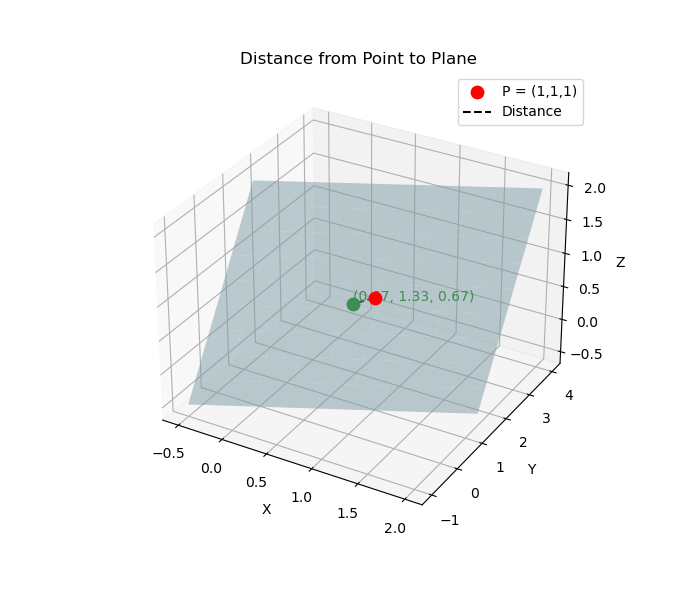
\includegraphics[height=0.5\textheight, keepaspectratio]{figs/Figure_1.png}
    \label{figure_1}
\end{figure}
\end{frame}

\begin{frame}[fragile]
    \frametitle{C Code}
    \begin{lstlisting}
#include <math.h>

double projection(const double *u1, const double *u2, const double *P, double *P_proj) {
    double U_TU[2][2], invU[2][2], UTP[2], coeff[2];

    // Compute Gram matrix U^T U
    U_TU[0][0] = u1[0]*u1[0] + u1[1]*u1[1] + u1[2]*u1[2];
    U_TU[0][1] = u1[0]*u2[0] + u1[1]*u2[1] + u1[2]*u2[2];
    U_TU[1][0] = U_TU[0][1];
    U_TU[1][1] = u2[0]*u2[0] + u2[1]*u2[1] + u2[2]*u2[2];

    double det = U_TU[0][0]*U_TU[1][1] - U_TU[0][1]*U_TU[1][0];
    invU[0][0] =  U_TU[1][1]/det;
    invU[0][1] = -U_TU[0][1]/det;
    invU[1][0] = -U_TU[1][0]/det;
    invU[1][1] =  U_TU[0][0]/det;



    \end{lstlisting}
\end{frame}
\begin{frame}[fragile]
    \frametitle{C Code}
    \begin{lstlisting}
    // Compute U^T P
    UTP[0] = u1[0]*P[0] + u1[1]*P[1] + u1[2]*P[2];
    UTP[1] = u2[0]*P[0] + u2[1]*P[1] + u2[2]*P[2];

    // Compute coefficients
    coeff[0] = invU[0][0]*UTP[0] + invU[0][1]*UTP[1];
    coeff[1] = invU[1][0]*UTP[0] + invU[1][1]*UTP[1];

    for(int i=0;i<3;i++)
        P_proj[i] = coeff[0]*u1[i] + coeff[1]*u2[i];

    double dist = 0.0;
    for(int i=0;i<3;i++)
        dist += (P[i] - P_proj[i]) * (P[i] - P_proj[i]);
    return sqrt(dist);
}

    \end{lstlisting}
\end{frame}

\begin{frame}[fragile]
    \frametitle{Python + C Code}
    \begin{lstlisting}
import ctypes
import numpy as np
import matplotlib.pyplot as plt
lib = ctypes.CDLL("./libdist.so")
lib.projection.argtypes = [
    np.ctypeslib.ndpointer(dtype=np.double, ndim=1, flags="C_CONTIGUOUS"),
    np.ctypeslib.ndpointer(dtype=np.double, ndim=1, flags="C_CONTIGUOUS"),
    np.ctypeslib.ndpointer(dtype=np.double, ndim=1, flags="C_CONTIGUOUS"),
    np.ctypeslib.ndpointer(dtype=np.double, ndim=1, flags="C_CONTIGUOUS")
]
lib.projection.restype = ctypes.c_double

    \end{lstlisting}
\end{frame}
\begin{frame}[fragile]
    \frametitle{Python + C Code}
    \begin{lstlisting}
u1 = np.array([1.0, 1.0, 0.0])
u2 = np.array([0.0, 1.0, 1.0])
P  = np.array([1.0, 1.0, 1.0])
P_proj = np.zeros(3, dtype=np.double)
# Compute projection and distance
distance = lib.projection(u1, u2, P, P_proj)
print(f"Distance from P to plane: {distance:.6f}")
print(f"Projection point: {P_proj}")

s = np.linspace(-0.5, 2, 10)
t = np.linspace(-0.5, 2, 10)
S, T = np.meshgrid(s, t)
X = S*u1[0] + T*u2[0]
Y = S*u1[1] + T*u2[1]
Z = S*u1[2] + T*u2[2]

fig = plt.figure(figsize=(7,6))
ax = fig.add_subplot(111, projection='3d')

    \end{lstlisting}
\end{frame}
\begin{frame}[fragile]
    \frametitle{Python + C Code}
    \begin{lstlisting}
ax.plot_surface(X, Y, Z, color='lightblue', alpha=0.5)
ax.scatter(*P, color='red', s=80, label='P = (1,1,1)')
ax.scatter(*P_proj, color='green', s=80)
ax.text(P_proj[0], P_proj[1], P_proj[2],
        f'({P_proj[0]:.2f}, {P_proj[1]:.2f}, {P_proj[2]:.2f})',
        color='green', fontsize=10, ha='left', va='bottom')
ax.plot([P[0], P_proj[0]], [P[1], P_proj[1]], [P[2], P_proj[2]], 'k--', label='Distance')

ax.set_xlabel('X')
ax.set_ylabel('Y')
ax.set_zlabel('Z')
ax.set_title('Distance from Point to Plane')
ax.legend()
plt.savefig("/mnt/c/Users/bharg/Documents/backupmatrix/ee25btech11013/matgeo/12.547/figs/Figure_1.png")
plt.show()
    \end{lstlisting}
\end{frame}


\begin{frame}[fragile]
    \frametitle{Python Code}
    \begin{lstlisting}
import numpy as np
import matplotlib.pyplot as plt

# Define vectors and point
u1 = np.array([1.0, 1.0, 0.0])
u2 = np.array([0.0, 1.0, 1.0])
P  = np.array([1.0, 1.0, 1.0])

# Stack u1 and u2 as columns to form U
U = np.column_stack((u1, u2))

# Compute projection coefficients: inv(U^T U) * U^T * P
coeff = np.linalg.inv(U.T @ U) @ (U.T @ P)

# Compute projection point
P_proj = U @ coeff


    \end{lstlisting}
\end{frame}
\begin{frame}[fragile]
    \frametitle{Python Code}
    \begin{lstlisting}
# Compute distance
distance = np.linalg.norm(P - P_proj)
print(f"Distance from P to plane: {distance:.6f}")
print(f"Projection point: {P_proj}")

# Create plane grid
s = np.linspace(-0.5, 2, 10)
t = np.linspace(-0.5, 2, 10)
S, T = np.meshgrid(s, t)
X = S*u1[0] + T*u2[0]
Y = S*u1[1] + T*u2[1]
Z = S*u1[2] + T*u2[2]

# Plotting
fig = plt.figure(figsize=(7,6))
ax = fig.add_subplot(111, projection='3d')

# Plane
ax.plot_surface(X, Y, Z, color='lightblue', alpha=0.5)

    \end{lstlisting}
\end{frame}
\begin{frame}[fragile]
    \frametitle{Python Code}
    \begin{lstlisting}
# Original point
ax.scatter(*P, color='red', s=80, label='P = (1,1,1)')
ax.scatter(*P_proj, color='green', s=80)
ax.text(P_proj[0], P_proj[1], P_proj[2],
        f'({P_proj[0]:.2f}, {P_proj[1]:.2f}, {P_proj[2]:.2f})',
        color='green', fontsize=10, ha='left', va='bottom')
ax.plot([P[0], P_proj[0]], [P[1], P_proj[1]], [P[2], P_proj[2]], 'k--', label='Distance')

ax.set_xlabel('X')
ax.set_ylabel('Y')
ax.set_zlabel('Z')
ax.set_title('Distance from Point to Plane')
ax.legend()
plt.savefig("/mnt/c/Users/bharg/Documents/backupmatrix/ee25btech11013/matgeo/12.547/figs/Figure_1.png")
plt.show()


    \end{lstlisting}
\end{frame}

\end{document}

